\chapter{Arhitektura i dizajn sustava}		
Arhitektura je podijeljena u tri podsustava:

\begin{itemize}
	\item Web poslužitelj
	\item Web aplikacija
	\item Baza podataka
\end{itemize}

\indent Internetski preglednik služi za pregled web-stranica i njihovog višemedijskog sadržaja, a one komuniciraju s poslužiteljima slanjem zahtjeva i primanjem odgovora. Preglednik ima sposobnost interpretacije koda kojim je pisana stranica u ljudski čitljiv oblik.
\newline
\indent Web poslužitelj je posrednik između korisnika i aplikacije, te služi kao osnova rada aplikacije. Komunikacija se ostvaruje korisničkim HTTP (engl. \textit{Hyper Text Transfer Protocol}) zahtjevima koji obično u zaglavlju imaju definiranu GET ili POST metodu za dohvaćanje odnosno predaju podataka. Poslužitelj na njih odgovara dostavom traženog sadržaja.
\newline
\indent Web aplikacija po nalogu poslužitelja pristupa ili mijenja podatke iz baze podataka i vraća HTML dokument koji se potom prikazuje korisniku u sučelju preglednika. Arhitektura sustava će se temeljiti na stilističkoj varijaciji arhitekture zasnovane na događajima (engl. \textit{event based architecture}) - MVC obrazcu. Spring - radni okvir korišten za razvoj pozadinskog dijela aplikacije, podržava MVC (Model-View-Controller) obrazac, te kao takav ima gotove predloške koji nam olakšavaju razvoj web aplikacije.
\newline

\clearpage
\indent MVC obrazac omogućuje odvojen razvoj navedenih slojeva aplikacije što znatno olakšava ispitivanje, razvijanje i dodavanje novih svojstava u sustav.
\newline
Dijelovi MVC obrazca su:
\begin{itemize}
	\item Model(\textit{Model}) - rješava problem interakcije korisnika s bazom podataka, predstavlja bazu i služi za komunikaciju upravljača s bazom, te je na taj način zadužen za logiku vezanu za podatke i njihov prijenos
	\item Prikaz(\textit{View}) - prikaz podataka i njihovih reprezentacija na korisničkom sučelju
	\item Upravljač(\textit{Controller}) - povezuje komponente modela i prikaza i služi kao posrednik između tih komponenata i korisnika, a sam nije zadužen za obradu podataka, međudjeluje s modelom kako bi dohvatio podatke i s prikazom kako bi ih prikazao korisniku
\end{itemize}

\begin{figure} [hbt!]
	
\includegraphics[width=\linewidth]{Slike/ArhitekturaSustava}
	\caption{Reprezentacija arhitekture sustava}
\end{figure}

		\clearpage

		\section{Baza podataka}
			
		Za potrebe našeg sustava koristit ćemo relacijsku bazu podataka koja svojom strukturom olakšava modeliranje stvarnog svijeta. Gradivna jedinka baze je relacija, odnosno tablica koja je definirana svojim imenom i skupom atributa. Zadaća baze podataka je brza i jednostavna pohrana, izmjena i dohvat podataka za daljnju obradu.
		Baza podataka ove aplikacije sastoji se od sljedećih entiteta: 
		
		\begin{itemize}
			\item Konferencija
			\item Korisnik
			\item Poster
			\item Pokrovitelj
			\item Pokrovitelj-Konferencije
			\item Fotografija
		\end{itemize}
		
		\clearpage
		
		\subsection{Opis tablica}
	
	\noindent\textbf{Konferencija }
	
	Ovaj entitet sadržava sve važne informacije o stručnoj konferenciji. Sadrži atribute: identifikator konferencije, ime konferencije, datum i vrijeme početka konferencije, datum i vrijeme završetka konferencije, mjesto održavanja konferencije, adresu održavanja konferencije, poštanski broj mjesta, generičko korisničko ime i pripadajuću lozinku koja se koristi za pristup konferenciji, poveznicu na video prijenos konferencije i oznaku o trajanju glasovanja. Ovaj entitet u vezi je \textit{jedan na više} s entitetom Korisnik preko identifikatora konferencije, u vezi \textit{jedan na više} s entitetom Poster preko identifikatora konferencije, u vezi \textit{jedan na više} s entitetom Fotografija preko identifikatora konferencije i u vezi \textit{više na više} s entitetom Pokrovitelj preko identifikatora konferencije. 
	
	\begin{longtblr}[
		label=none,
		entry=none
		]{
			width = \textwidth,
			colspec={|X[6,l]|X[6, l]|X[20, l]|}, 
			rowhead = 1,
		} %definicija širine tablice, širine stupaca, poravnanje i broja redaka naslova tablice
		\hline \SetCell[c=3]{c}{\textbf{Konferencija}}	 \\ \hline[3pt]
		\SetCell{LightGreen}id\_konferencija & INT	&  	jedinstveni brojčani identifikator konferencije  	\\ \hline
		ime\_ konferencija	& VARCHAR &   jedinstveno ime konferencije	\\ \hline 
		datum\_vrijeme \_pocetka & TIMESTAMP & datum i vrijeme početka konferencije  \\ \hline
		datum\_vrijeme \_zavrsetka & TIMESTAMP & datum i vrijeme završetka konferencije \\ \hline
		mjesto	& VARCHAR & ime mjesta u kojem se održava konferencija \\ \hline 
		adresa & VARCHAR & adresa održavanja konferencije \\ \hline
		zip\_code & VARCHAR & poštanski broj mjesta održavanja konferencije \\ \hline
		generic\_ username	& VARCHAR & generičko korisničko ime koje koriste svi posjetitelji konferencije prije izrade vlastitog korisničkog računa  \\ \hline 
		generic\_ password & VARCHAR & hash lozinka generičkog korisničkog računa \\ \hline
		video\_url & VARCHAR & poveznica na video prijenos konferencije \\ \hline
		voting\_ reminder\_sent & BOOLEAN & oznaka pomoću koje aplikacija svakih 24 sata provjerava traje li glasanje za zadanu konferenciju \\ \hline
	\end{longtblr}
	
	\clearpage
	
	\noindent\textbf{Korisnik }
	
	Ovaj entitet sadržava sve važne informacije o korisniku aplikacije. Sadrži atribute: identifikator korisnika, e-mail adresu korisnika, lozinku, ime, prezime, oznaku ima li korisnik ovlasti administratora, oznaku radi li se o generičkom računu, oznaku je li korisnik glasao i identifikator konferencije na kojoj korisnik sudjeluje.  Ovaj entitet je u vezi \textit{više na jedan} s entitetom Konferencija preko identifikatora konferencije. 
	
	\begin{longtblr}[
		label=none,
		entry=none
		]{
			width = \textwidth,
			colspec={|X[6,l]|X[6, l]|X[20, l]|}, 
			rowhead = 1,
		} %definicija širine tablice, širine stupaca, poravnanje i broja redaka naslova tablice
		\hline \SetCell[c=3]{c}{\textbf{Korisnik}}	 \\ \hline[3pt]
		\SetCell{LightGreen}id\_korisnik & INT &  jedinstveni brojčani identifikator korisnika	\\ \hline
		email & VARCHAR	&  e-mail adresa kojom korisnik izrađuje korisnički račun 	\\ \hline
		lozinka	& VARCHAR & hash lozinka korisničkog računa  	\\ \hline 
		ime & VARCHAR & ime korisnika  \\ \hline 
		prezime & VARCHAR	& prezime korisnika 		\\ \hline 
		admin & BOOLEAN &  oznaka ima li ovlasti administratora		\\ \hline 
		visitor & BOOLEAN &  oznaka radi li se o generičkom računu (TRUE), kada posjetitelj napravi vlastiti korisnički račun vrijednost varijable postaje FALSE	\\ \hline 
		voted & BOOLEAN & oznaka je li korisnik glasao \\ \hline
		\SetCell{LightBlue} id\_konferencija	& INT & jedinstveni identifikator konferencije na kojoj korisnik sudjeluje (konferencija.id\_konferencija)  	\\ \hline 
	\end{longtblr}
	
	\clearpage
	
	\noindent \textbf{Poster }
	
	Ovaj entitet sadržava sve važne informacije o radu prikazanom odgovarajućim posterom/prezentacijom. Sadrži atribute: identifikator postera, ime postera, datoteku postera, broj glasova za poster, ime i prezime autora, e-mail adresu kojom je autor poslao poster i identifikator konferencije na kojoj se rad izlaže. Ovaj entitet je u vezi \textit{više na jedan} s entitetom Konferencija preko identifikatora konferencije.
	
	
	\begin{longtblr}[
		label=none,
		entry=none
		]{
			width = \textwidth,
			colspec={|X[6,l]|X[6, l]|X[20, l]|}, 
			rowhead = 1,
		} %definicija širine tablice, širine stupaca, poravnanje i broja redaka naslova tablice
		\hline \SetCell[c=3]{c}{\textbf{Poster}}	 \\ \hline[3pt]
		\SetCell{LightGreen}id\_poster & INT &  jedinstveni brojčani identifikator postera	\\ \hline
		ime\_poster & VARCHAR	&  ime postera\\ \hline
		file\_path & LONGBLOB & PDF datoteka postera ili prezentacije  \\ \hline 
		br\_glasova & INT & broj glasova za određeni poster \\ \hline 
		ime\_autor & VARCHAR & ime autora \\ \hline
		prezime\_autor & VARCHAR & prezime autora \\ \hline
		poster\_email & VARCHAR & e-mail adresa autora \\ \hline
		\SetCell{LightBlue} id\_konferencija	& INT & jedinstveni brojčani identifikator konferencije kojoj poster pripada (konferencija.id\_konferencija)  	\\ \hline 
	\end{longtblr}
	
	\clearpage
	
	\noindent \textbf{Pokrovitelj }
	
	Ovaj entitet sadržava sve važne informacije o pokrovitelju. Sadrži atribute: identifikator pokrovitelja, ime pokrovitelja, promotivne materijale i poveznicu na stranicu pokrovitelja. Ovaj entitet je u vezi \textit{više na više} s entitetom Konferencija.
	
	
	\begin{longtblr}[
		label=none,
		entry=none
		]{
			width = \textwidth,
			colspec={|X[6,l]|X[6, l]|X[20, l]|}, 
			rowhead = 1,
		} %definicija širine tablice, širine stupaca, poravnanje i broja redaka naslova tablice
		\hline \SetCell[c=3]{c}{\textbf{Pokrovitelj}}	 \\ \hline[3pt]
		\SetCell{LightGreen}id\_pokrovitelj & INT & jedinstveni brojčani identifikator pokrovitelja  	\\ \hline
		ime\_ pokrovitelja & VARCHAR & jedinstveni identifikator pokrovitelja  	\\ \hline
		promotivni\_ materijal & LONGBLOB & datoteka, promotivni materijal je logotip pokrovitelja   \\ \hline 
		url\_promo & VARCHAR & poveznica na stranicu pokrovitelja \\ \hline 
	\end{longtblr}
	
	\noindent \textbf{Pokrovitelj-Konferencije }
	
	Ovaj entitet nastaje zbog \textit{više na više} veze između entiteta Konferencija i Pokrovitelj. Sadržava sve informacije o odnosu konferencije i pokrovitelja odnosno kojoj konferenciji pokrovitelj pripada. 
	
	
	\begin{longtblr}[
		label=none,
		entry=none
		]{
			width = \textwidth,
			colspec={|X[6,l]|X[6, l]|X[20, l]|}, 
			rowhead = 1,
		} %definicija širine tablice, širine stupaca, poravnanje i broja redaka naslova tablice
		\hline \SetCell[c=3]{c}{\textbf{Pokrovitelj-Konferencije}}	 \\ \hline[3pt]
		\SetCell{LightBlue} id\_pokrovitelj	& INT & jedinstveni brojčani identifikator pokrovitelja (pokrovitelj.id\_pokrovitelj)     	\\ \hline
		\SetCell{LightBlue}id\_konferencija	& INT & jedinstveni brojčani identifikator konferencije (konferencija.id\_konferencija)  	\\ \hline 
		
	\end{longtblr}
	
	
	\noindent \textbf{Fotografija }
	
	Ovaj entitet sadržava sve informacije o fotografijama s konferencije. Sadrži atribute: identifikator fotografije, sliku fotografije i identifikator konferencije kojoj fotografija pripada. Ovaj entitet u vezi je \textit{više na jedan} s entitetom Konferencija. 
	
	
	\begin{longtblr}[
		label=none,
		entry=none
		]{
			width = \textwidth,
			colspec={|X[6,l]|X[6, l]|X[20, l]|}, 
			rowhead = 1,
		} %definicija širine tablice, širine stupaca, poravnanje i broja redaka naslova tablice
		\hline \SetCell[c=3]{c}{\textbf{Fotografije}}	 \\ \hline[3pt]
		\SetCell{LightGreen}id\_fotografija & INT & jedinstveni brojčani identifikator fotografije   	\\ \hline
		file\_path	& LONGBLOB &  fotografije	\\ \hline 
		\SetCell{LightBlue} id\_konferencija	& INT & jedinstveni brojčani identifikator konferencije kojoj fotografija pripada (konferencija.id\_konferencija)	\\ \hline 
	\end{longtblr}
	
	\clearpage
			
			\subsection{Dijagram baze podataka}
				
					\begin{figure} [h]
						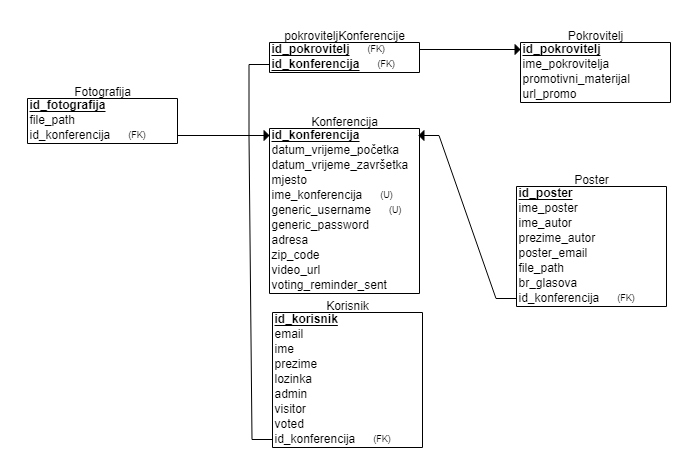
\includegraphics[width=\linewidth]{Slike/ERDijagramFinal}
						\caption{E-R dijagram baze podataka}
					\end{figure}
			
			\eject
			
			
		\section{Dijagram razreda}
			
			\indent Slike 4.3, 4.4 i 4.5 prikazuju dijagrame razreda pozadinskog dijela MVC arhitekture. Slike 4.3 i 4.4 prikazuju upravljačke razrede, te DAO (\textit{Data Access Object} razrede. 
			
			Dijagrami su zbog preglednosti podijeljeni po slojevima, odnosno na pojedinom dijagramu prikazane su samo ovisnosti između razreda istog MVC sloja, a prema nazivima samih razreda može se logički zaključiti koji su razredi različitih slojeva funkcionalno povezani.
			
			Razredi dijagrama na slici 4.5 preslikavaju entitete i atribute baze podataka. Razred Korisnik predstavlja općeniti model korisnika aplikacije koji može biti posjetitelj konferencije ili administrator. Može se registrirati u sustav unoseći osnove informacije. Razred Konferencija predstavlja skup podataka koji su potrebni za registraciju konferencije i koji se prikazuju korisnicima. Razred Poster predstavlja skup podataka koji su potrebni za dodavanje postera i koji se prikazuju korisnicima. Razred Fotografija predstavlja skup podataka vezan uz pojedinačnu fotografiju konferencije. Razred Pokrovitelj predstavlja pokrovitelja konferencije.
			
			\begin{figure} [hbt!]
				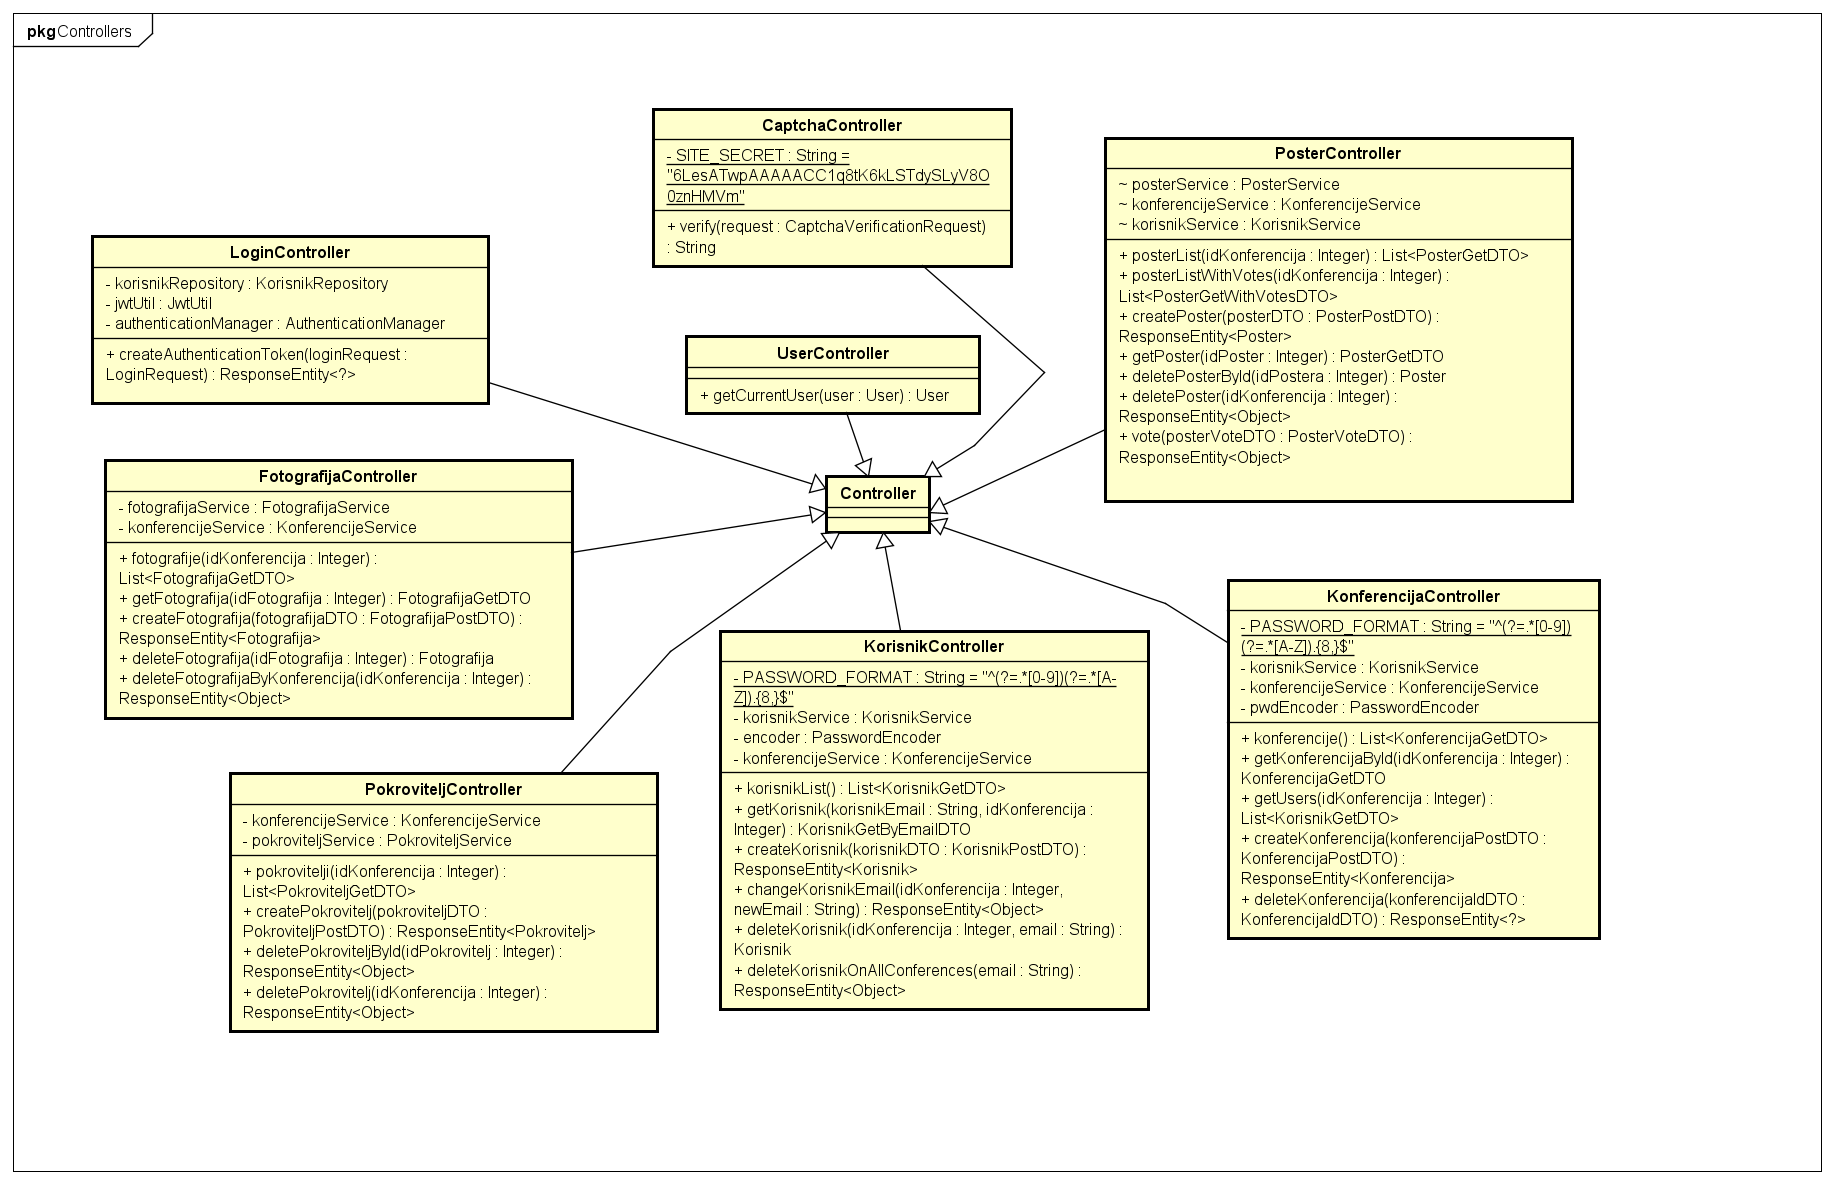
\includegraphics[width=\linewidth]{Slike/Controllers}
				\caption{Dijagram razreda - Upravljači}
			\end{figure}
			
			\begin{figure} [hbt!]
				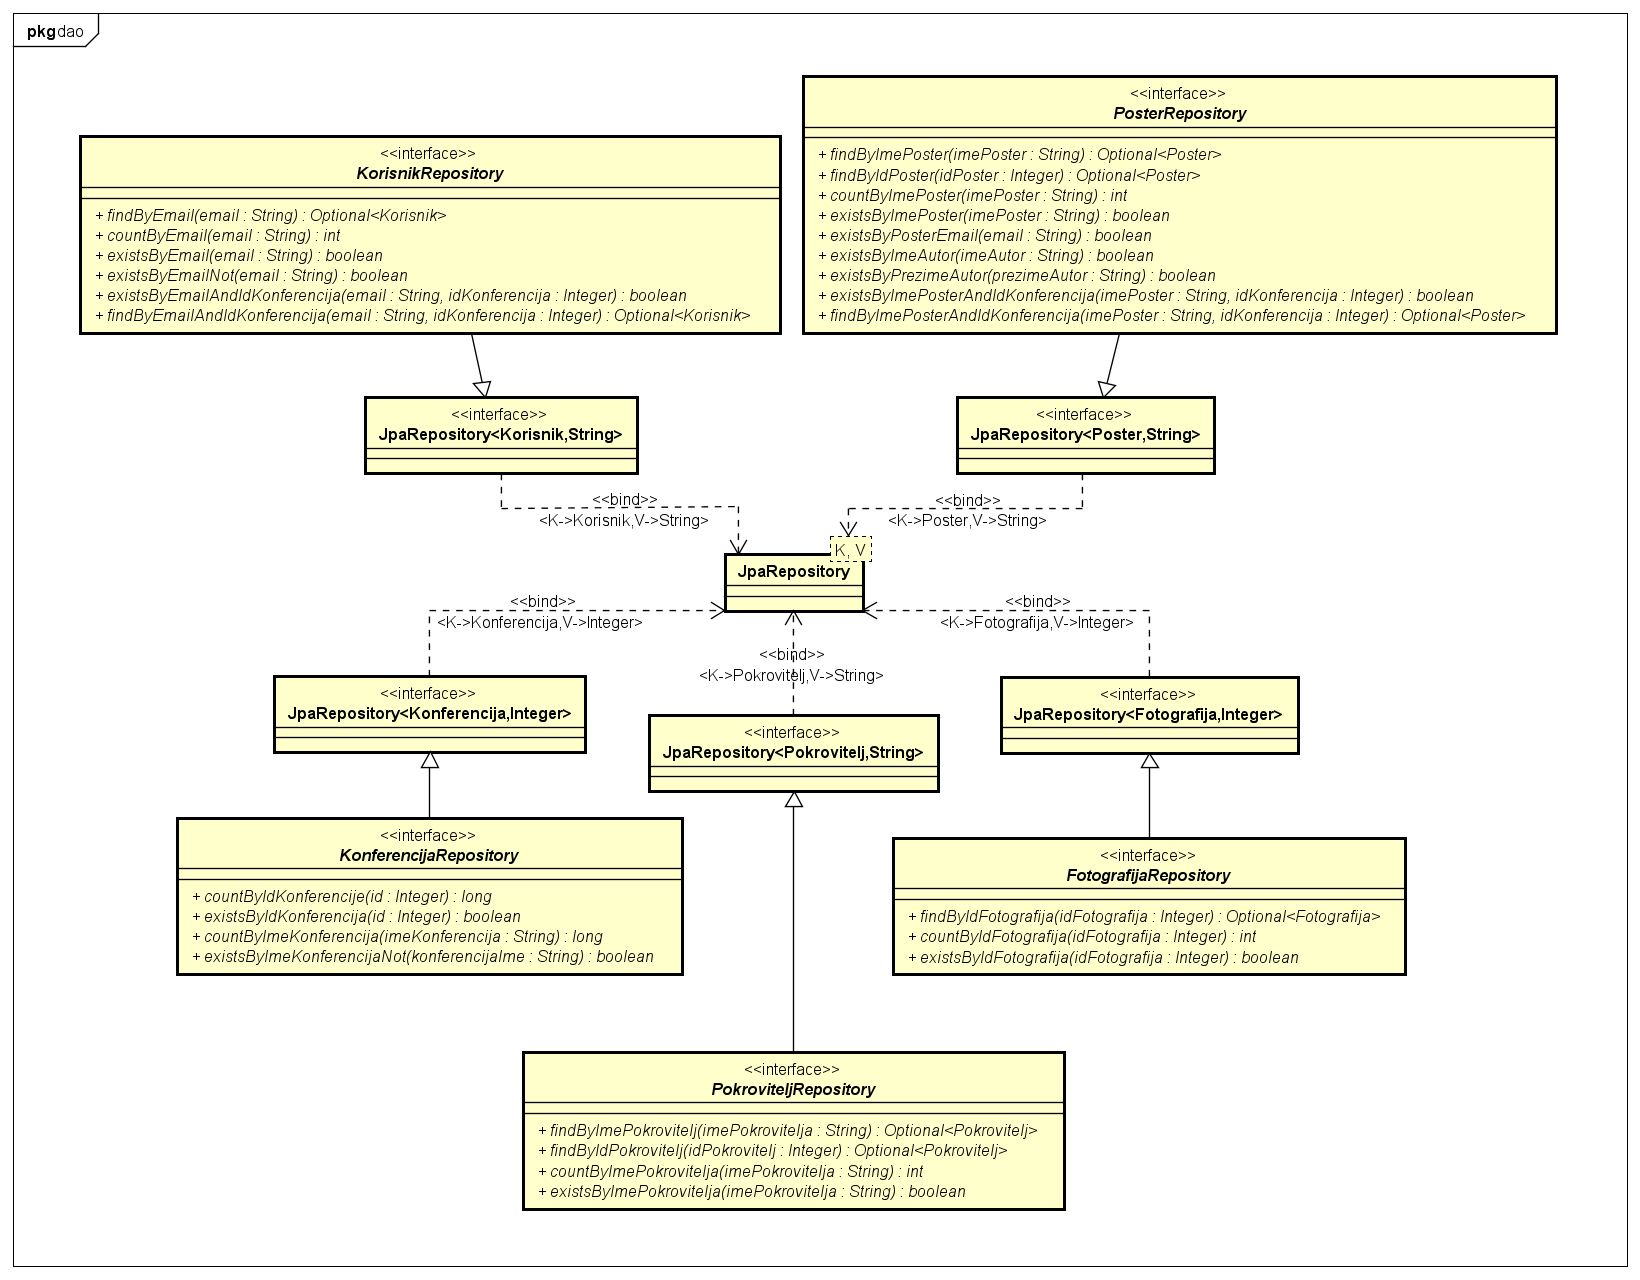
\includegraphics[width=\linewidth]{Slike/ClassDiagramDAORevised}
				\caption{Dijagram razreda - DAO}
			\end{figure}
			
			\begin{figure} [hbt!]
				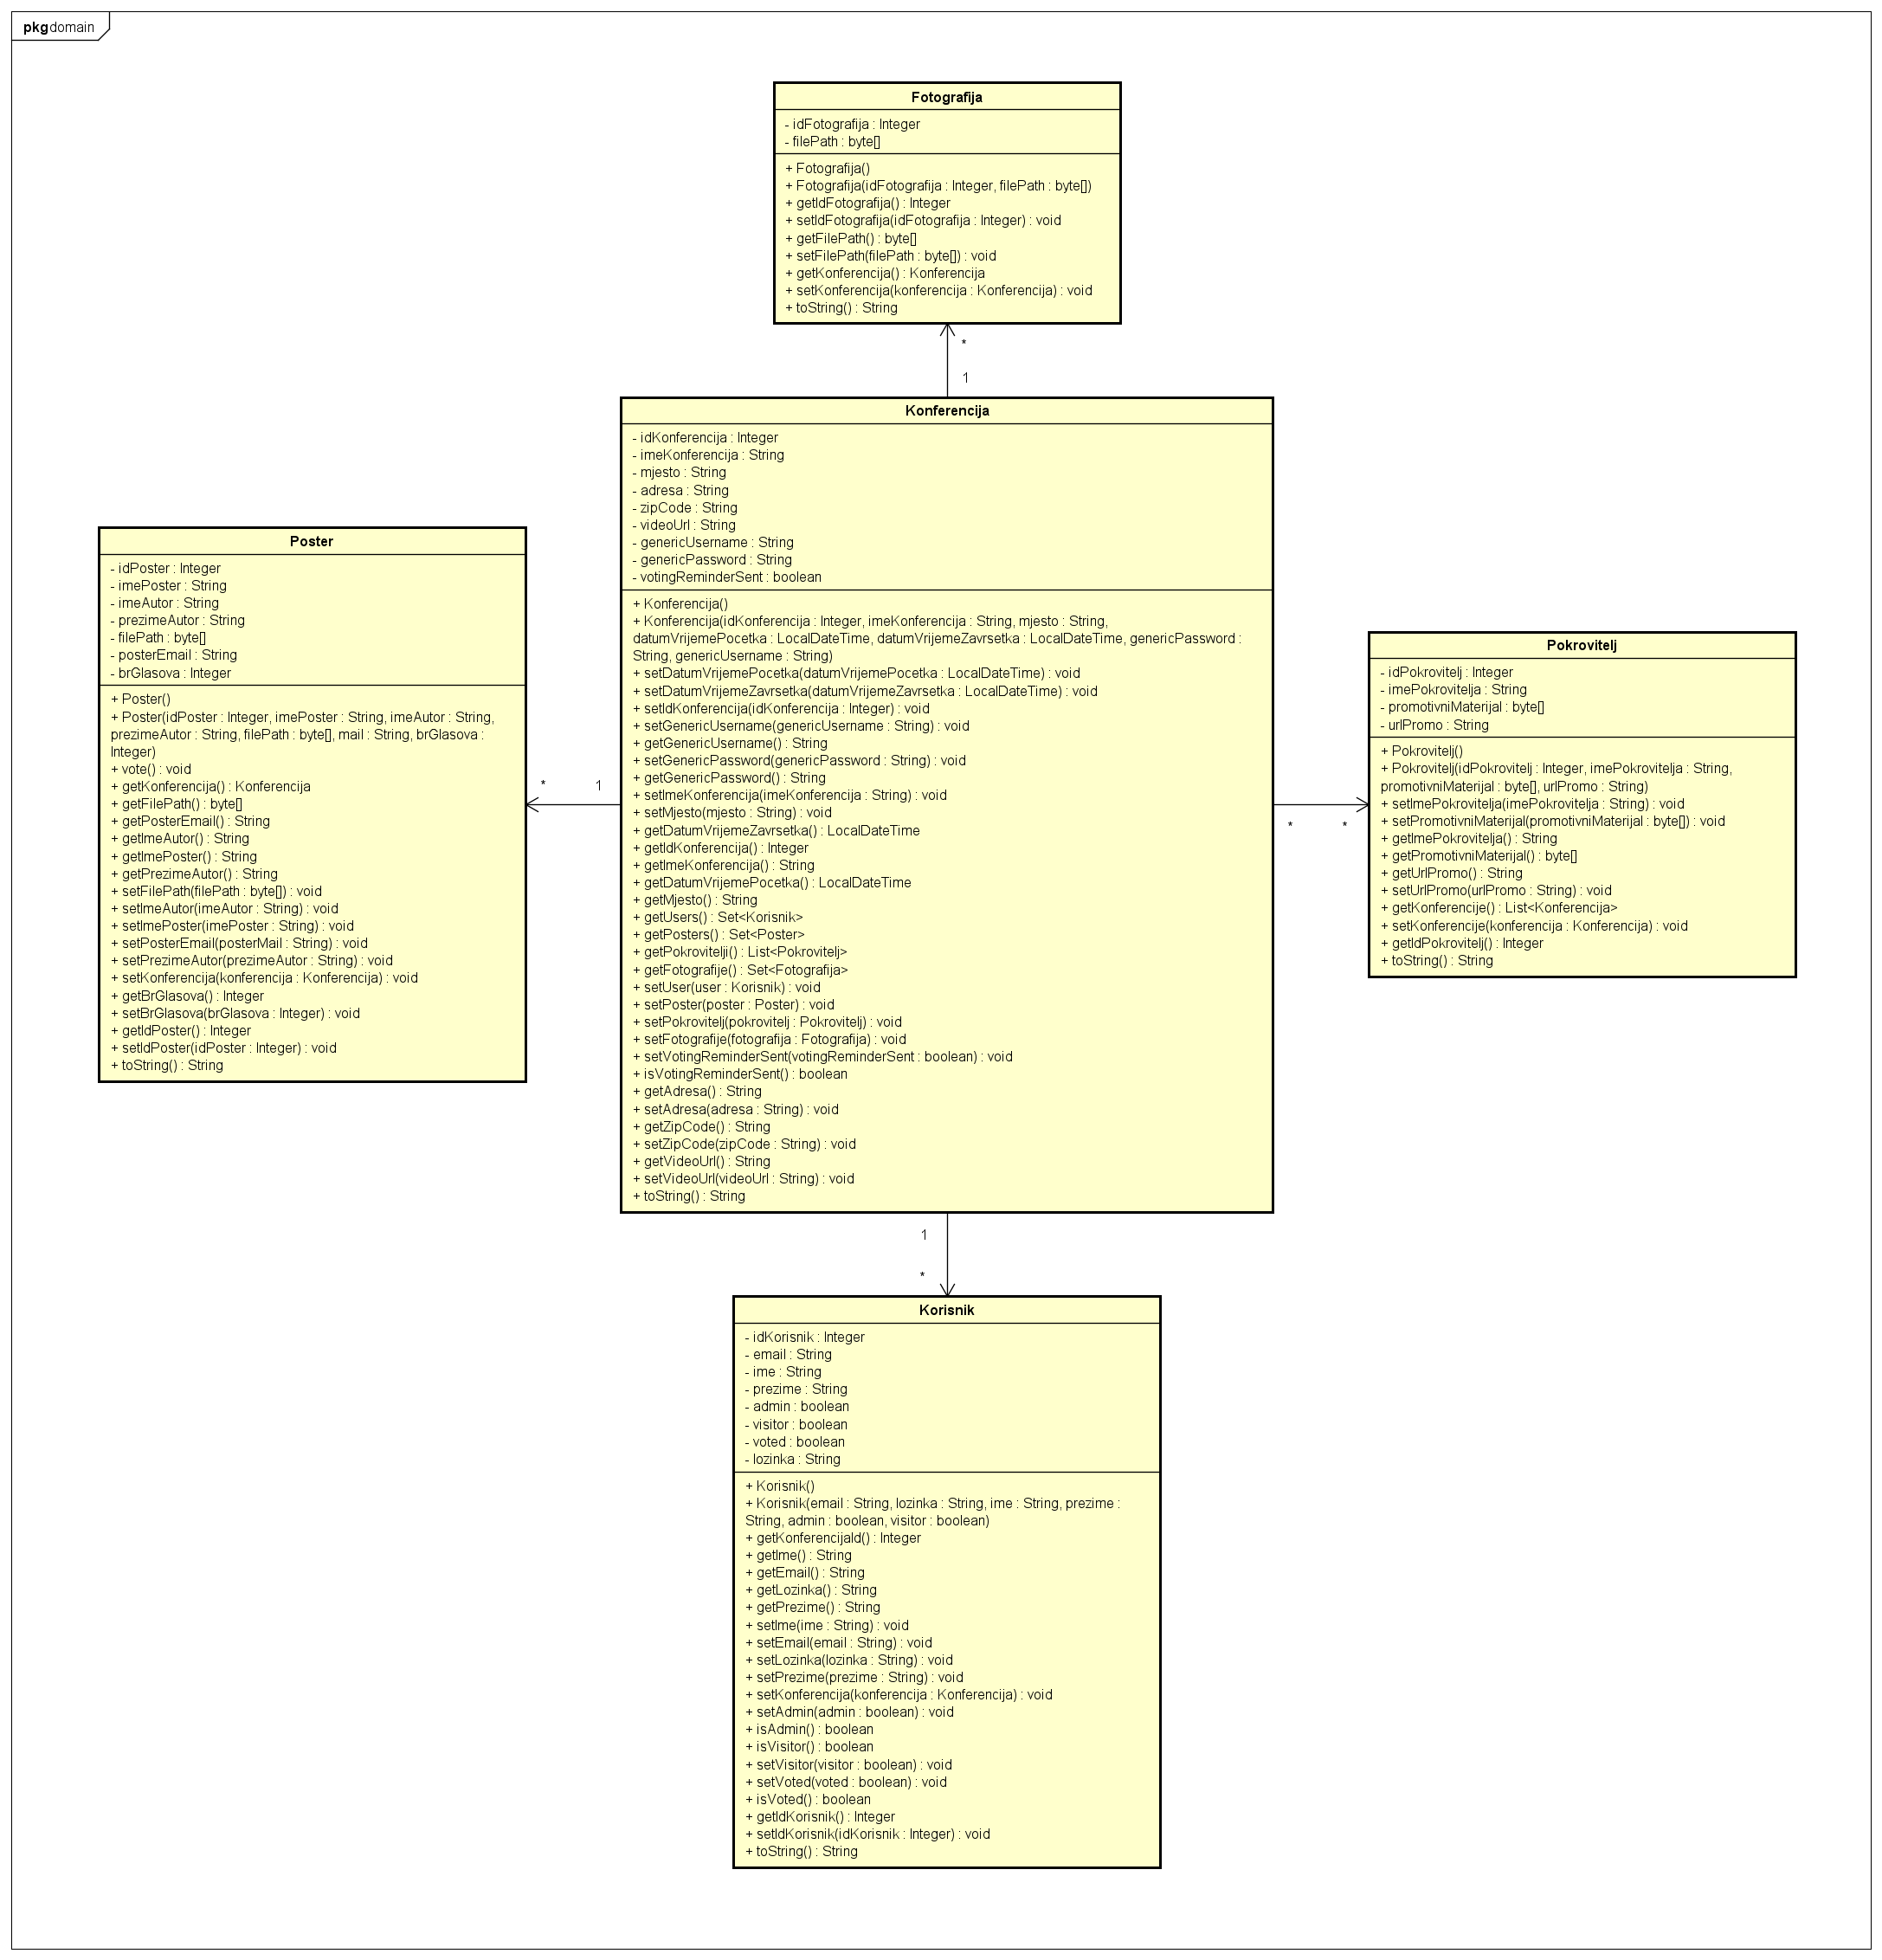
\includegraphics[width=\linewidth]{Slike/ClassDiagramModelsRevised}
				\caption{Dijagram razreda - Modeli}
			\end{figure}
			
			\clearpage
			 
			\textbf{\textit{dio 2. revizije}}\\			
			
			\textit{Prilikom druge predaje projekta dijagram razreda i opisi moraju odgovarati stvarnom stanju implementacije}
			
			
			
			\eject
		
		\section{Dijagram stanja}
			
			
			\textbf{\textit{dio 2. revizije}}\\
			
			\textit{Potrebno je priložiti dijagram stanja i opisati ga. Dovoljan je jedan dijagram stanja koji prikazuje \textbf{značajan dio funkcionalnosti} sustava. Na primjer, stanja korisničkog sučelja i tijek korištenja neke ključne funkcionalnosti jesu značajan dio sustava, a registracija i prijava nisu. }
			
			\indent Dijagram stanja opisuje ponašanje sustava koristeći konačan broj apstraktnih diskretnih stanja u kojima se on može nalaziti i načine na koje se može prijeći iz jednog u drugo stanje, odnosno korisničke akcije koje potiču te prijelaze. Na slici 4.6 je prikazan dijagram stanja za registriranog korisnika koji je prije same registracije pristupio konferenciji pomoću generičke lozinke. Registriranom korisniku omogućen je pregled samo onih konferencija kojima je pristupio. Nakon uspješnog pristupa konferenciji, korisniku se prikazuje početna stranica konferencije na kojoj može pregledati vrijeme i mjesto događaja, vremensku prognozu za idućih 48 sati na toj lokaciji, te video prijenos konferencije, kao i popis pokrovitelja konferencije. Navigacijska traka korisniku omogućava pristup posterima, fotografijama, te pokroviteljima konferencije. Klikom na "Posteri" prikazuje mu se galerija postera gdje ima mogućnost glasanja za poster po izboru unutar zadanog vremenskog ograničenja. Klikom na "Fotografije" otvara se galerija fotografija, odakle se odabrane fotografije mogu preuzeti na računalo. Klikom na "Pokrovitelji", korisniku se prikazuju pokrovitelji konferencije. Klikom na logo određenog pokrovitelja otvoriti će se službena stranica pokrovitelja koja se nalazi izvan aplikacije. Nakon završetka glasovanja korisnik će imati pristup rezultatima klikom na "Rezultati".
			
			\begin{figure} [hbt!]
				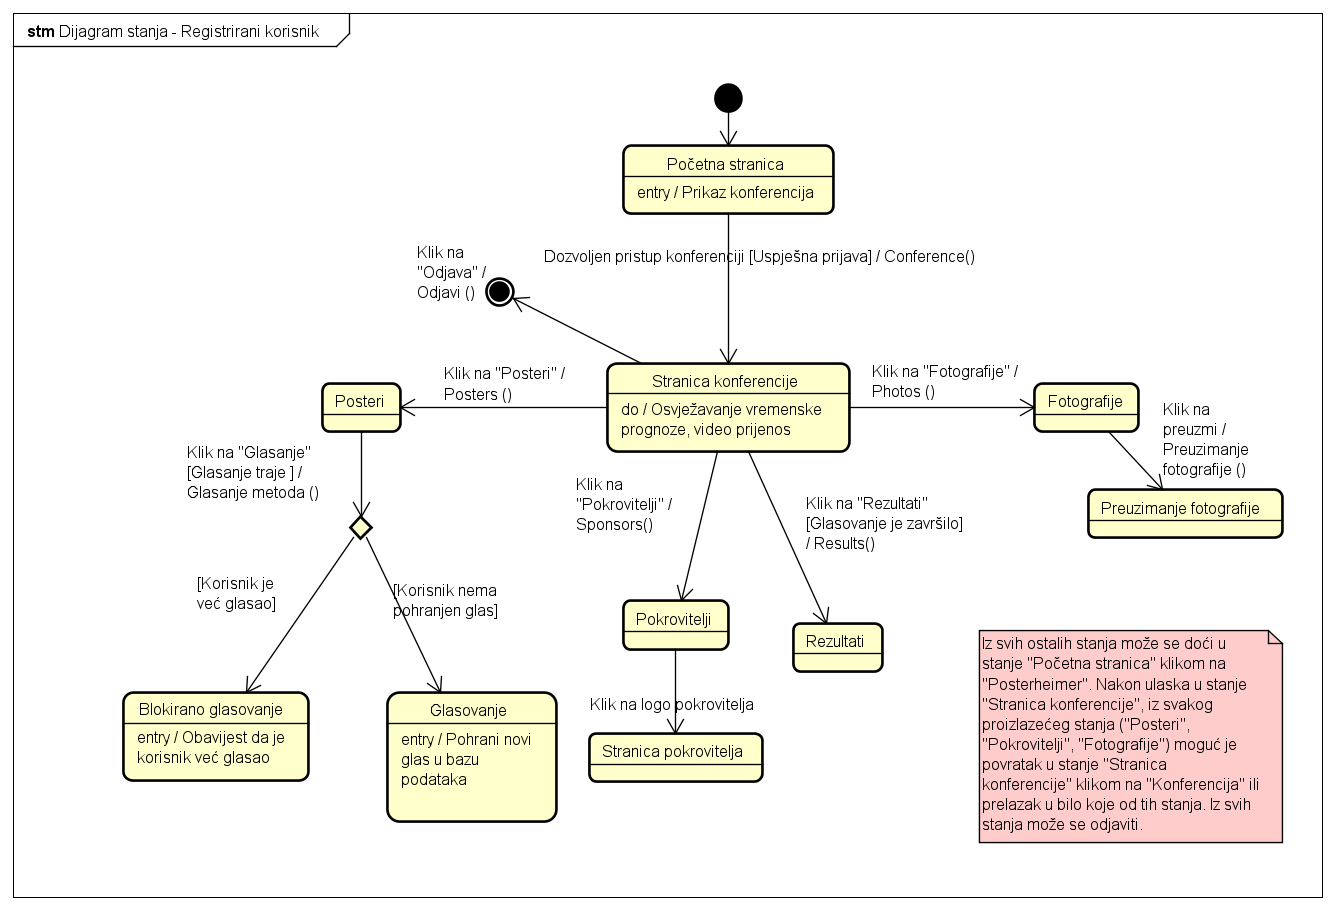
\includegraphics[width=\linewidth]{Slike/StateMachineDiagram}
				\caption{Dijagram stanja}
			\end{figure}
			
			
			\eject 
		
		\section{Dijagram aktivnosti}
			
			\textbf{\textit{dio 2. revizije}}\\
			
			 \textit{Potrebno je priložiti dijagram aktivnosti s pripadajućim opisom. Dijagram aktivnosti treba prikazivati značajan dio sustava.}
			 
			 \indent Dijagram aktivnosti opisuje ponašanje funkcionalnog dijela sustava, te interakciju više fizički ili programski odvojenih dijelova sustava, a posebno je pogodan za prikaz njihove sinkronizacije i konkurentnog djelovanja. Dijagram aktivnosti na slici 4.7 prikazuje tok podataka postupka glasovanja za poster. Korisnik pristupa aplikaciji i odabire konferenciju na kojoj sudjeluje. Klikom na opciju "Posteri" korisniku će se prikazati galerija postera. Korisnik odabire jedan poster te za njega glasa.    
			 
			 \begin{figure}
			 	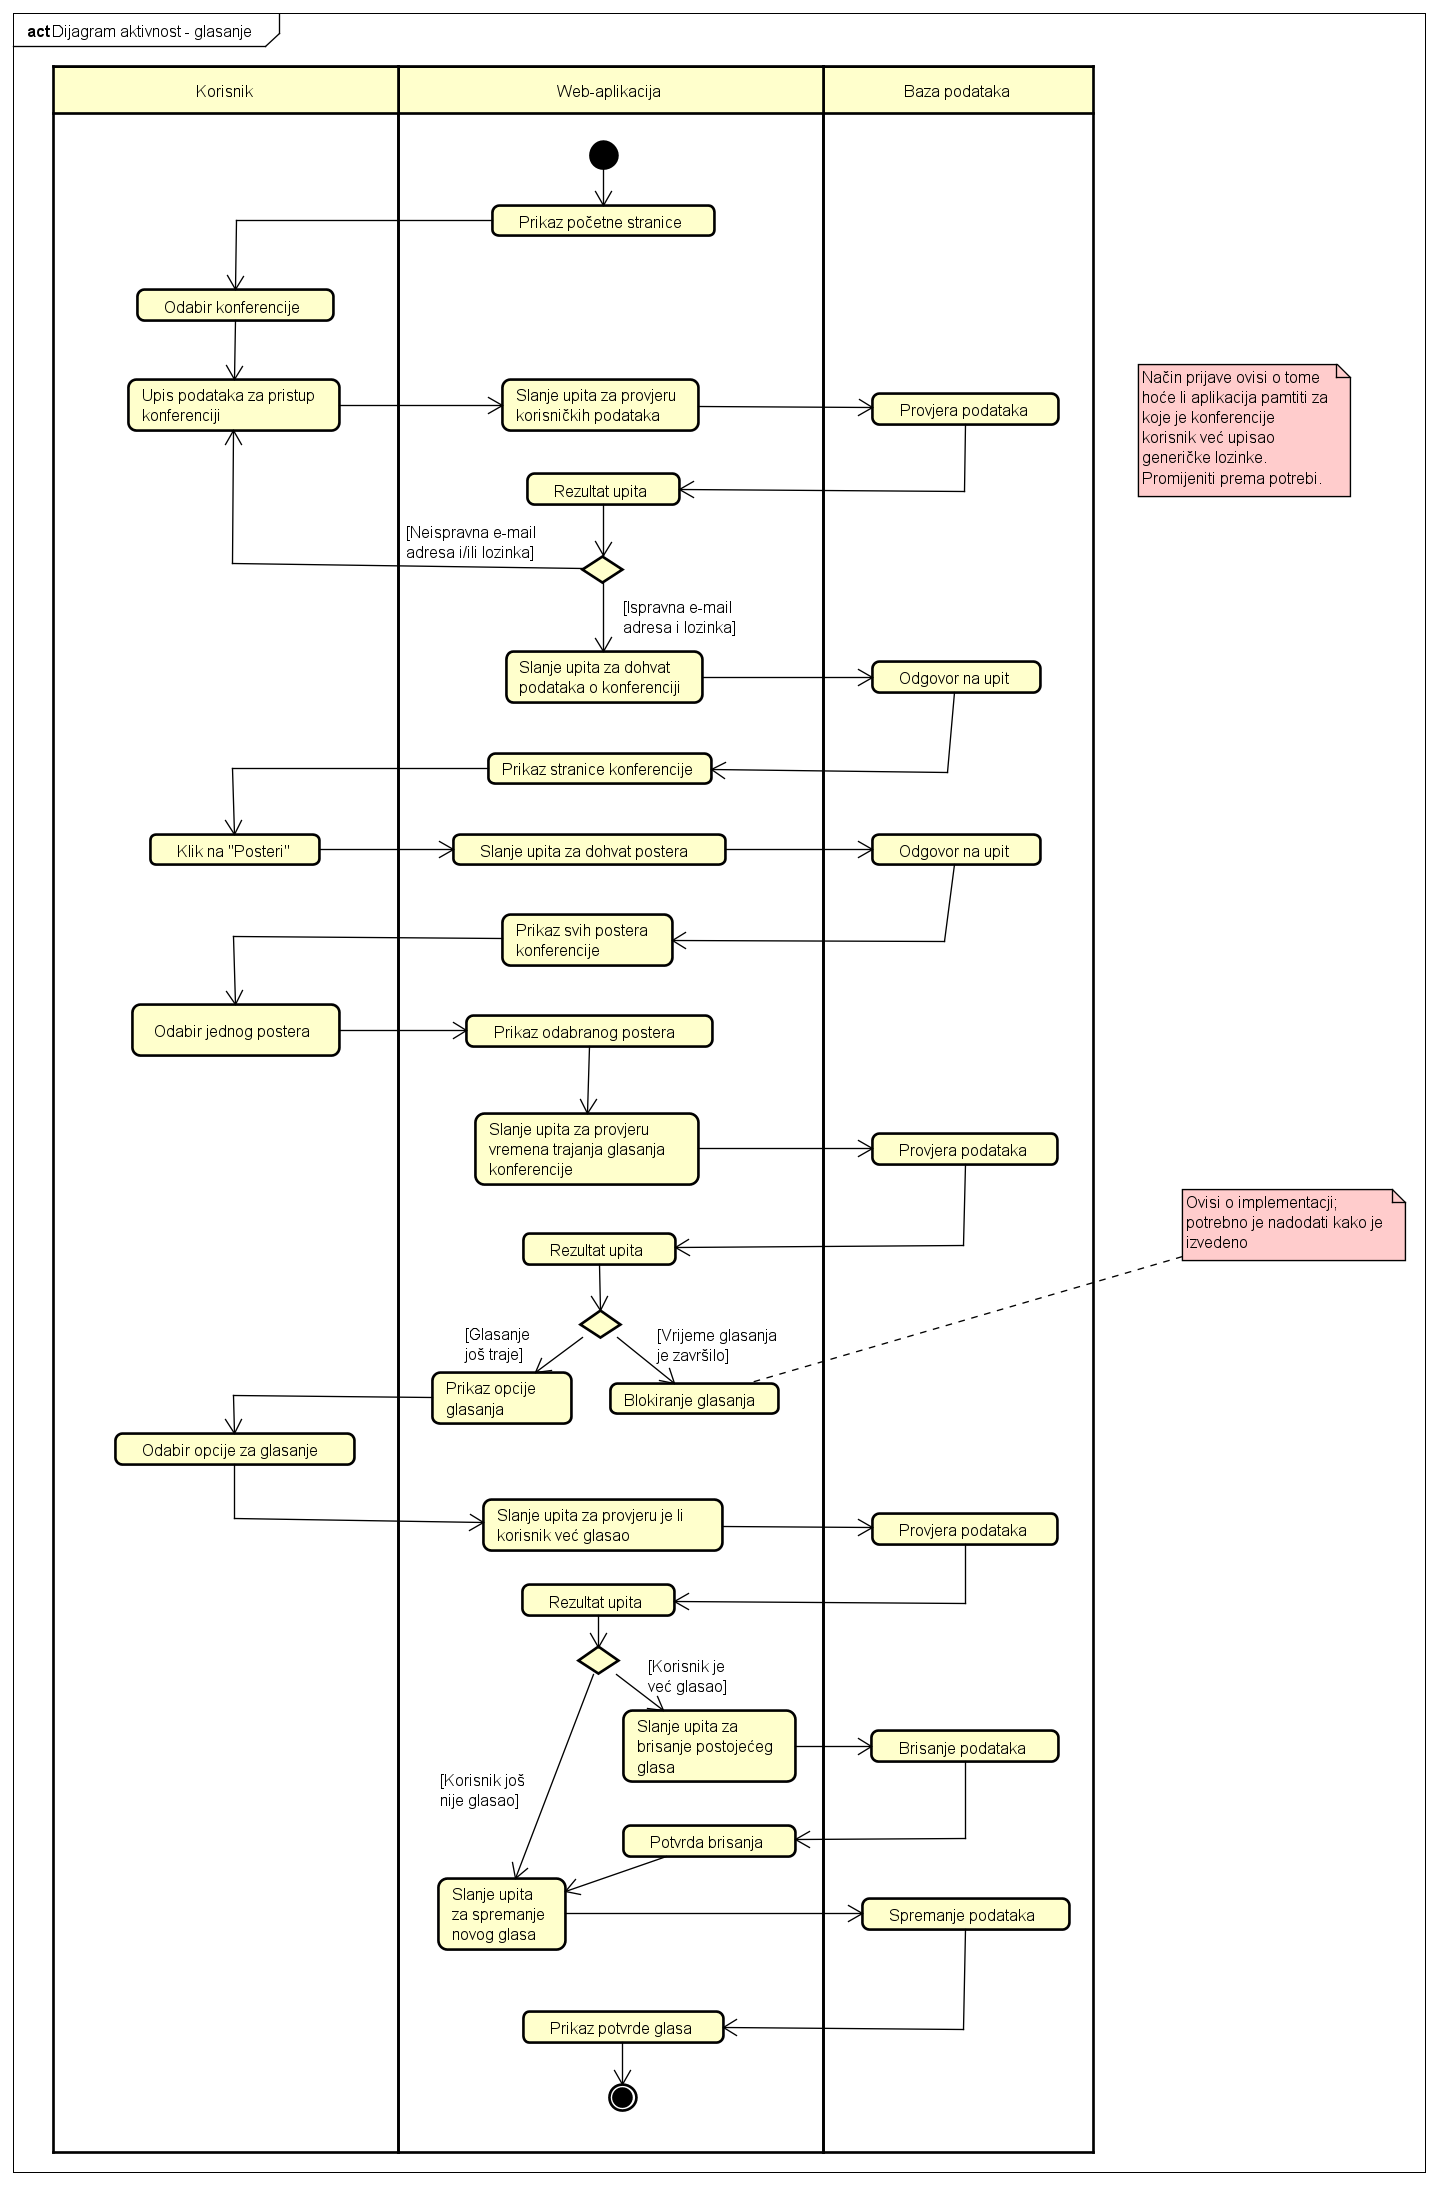
\includegraphics[width=\linewidth]{Slike/ActivityDiagram}
			 	\caption{Dijagram aktivnosti - Glasovanje}
			 \end{figure}
			
			\eject
		\section{Dijagram komponenti}
		
			\textbf{\textit{dio 2. revizije}}\\
		
			 \textit{Potrebno je priložiti dijagram komponenti s pripadajućim opisom. Dijagram komponenti treba prikazivati strukturu cijele aplikacije.}
			 
			 \indent Dijagram komponenti prikazan na slici 4.8 vizualizira organizaciju programskih komponenti i cjelina, te njihovu međuovisnost i međusobnu interakciju preko nuđenih i traženih sučelja. Sustavu se pristupa preko dva različita sučelja. Preko sučelja za dohvat HTML, CSS i JSX datoteka poslužuju se datoteke koje pripadaju prednjem \textit{engl. frontend} dijelu aplikacije. AppRouter je komponenta koja na upit s url određuje koja datoteka će se poslužiti na sučelje. Prednji \textit{engl. frontend} dio sastoji se od niza JavaScript XML datoteka koje su raspoređene u logičke cjeline nazvane po dijelu aplikacije za koji se koriste. Sve JavaScript XML datoteke ovise o React biblioteci iz koje dohvaćaju gotove komponente. Preko sučelja za dohvat JSON podataka pristupa se REST API komponenti. REST API poslužuje podatke koji pripadaju \textit{backend} dijelu aplikacije. Repository je zadužen za dohvaćanje tablica iz baze podataka pomoću SQL upita. Podaci koji su pristigli iz baze se šalju dalje MVC arhitekturi u obliku DTO \textit{(Data transfer object)}. React-view komponenta preko dostupnih sučelja komunicira sa Posterheimer aplikacijom te ovisno o korisnikovim akcijama osvježava prikaz i dohvaća nove podatke ili datoteke.
			 
			 \begin{figure}
			 	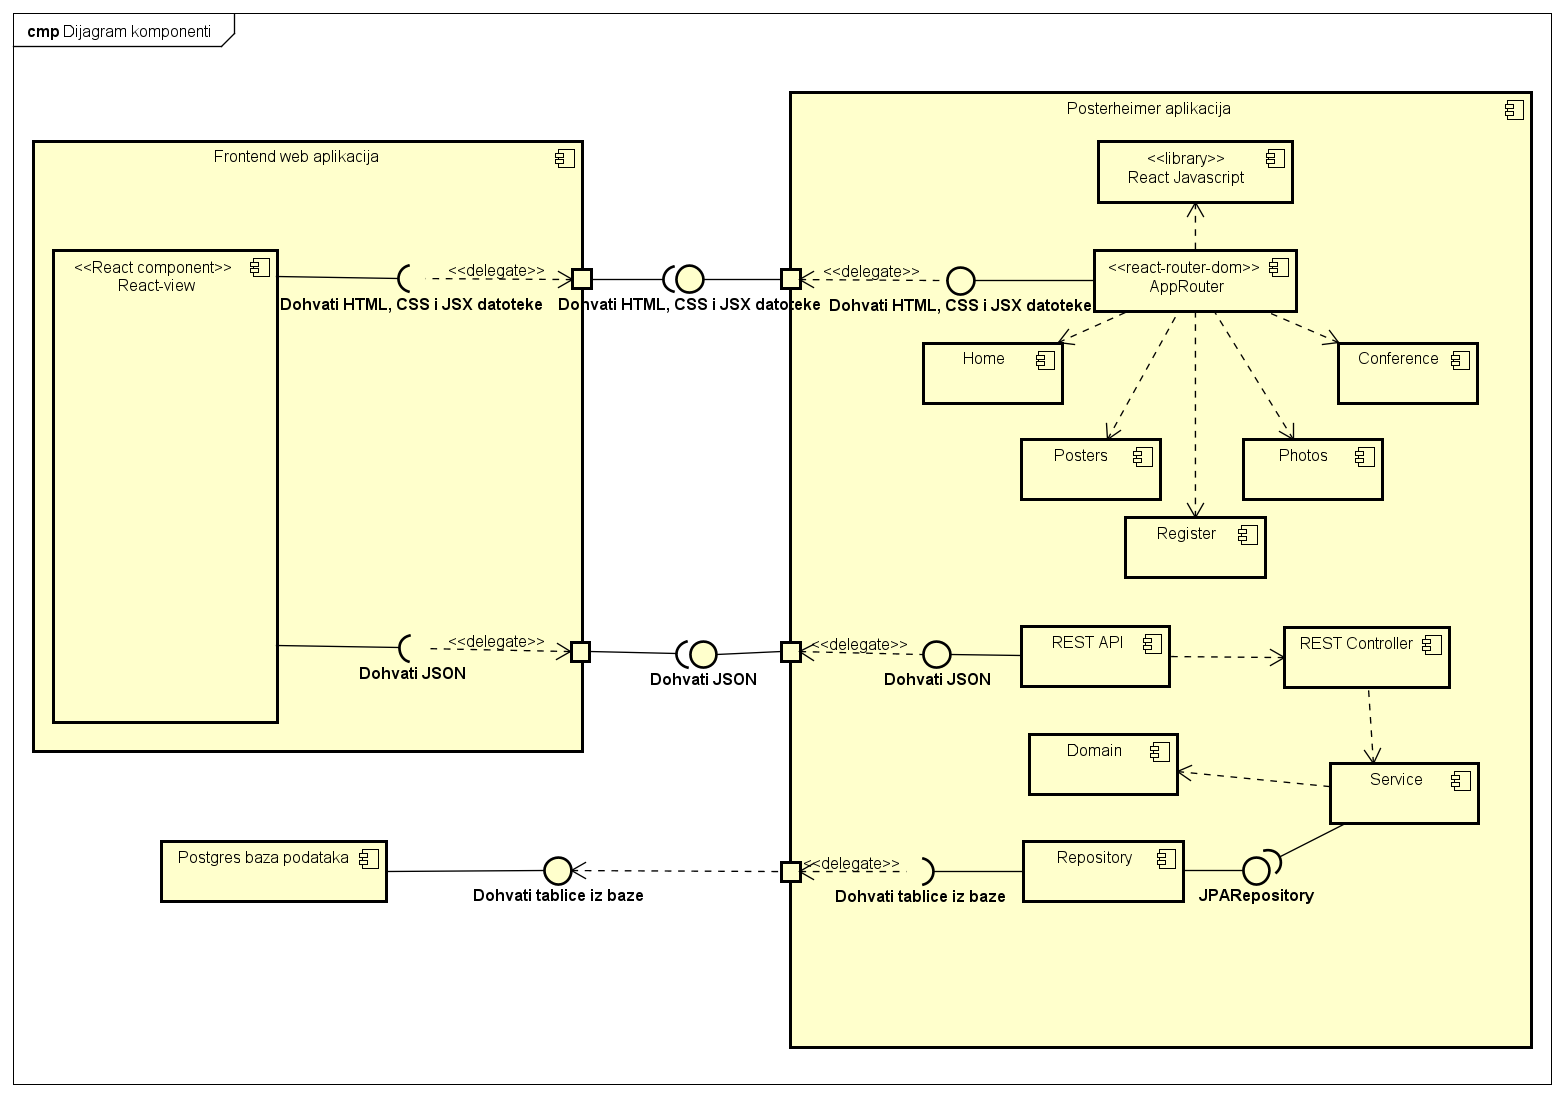
\includegraphics[width=\linewidth]{Slike/ComponentDiagram}
			 	\caption{Dijagram komponenti}
			 \end{figure}